\begin{figure}[t!] % [H] for no float
\captionsetup{justification=raggedright,singlelinecheck=true}
\caption{Brazil--U.S. soybean landed price with tariff in China differential by week and U.S. weekly net export sales to China.}
\label{fig:price_spread}
\begin{threeparttable}
% --- chart ---
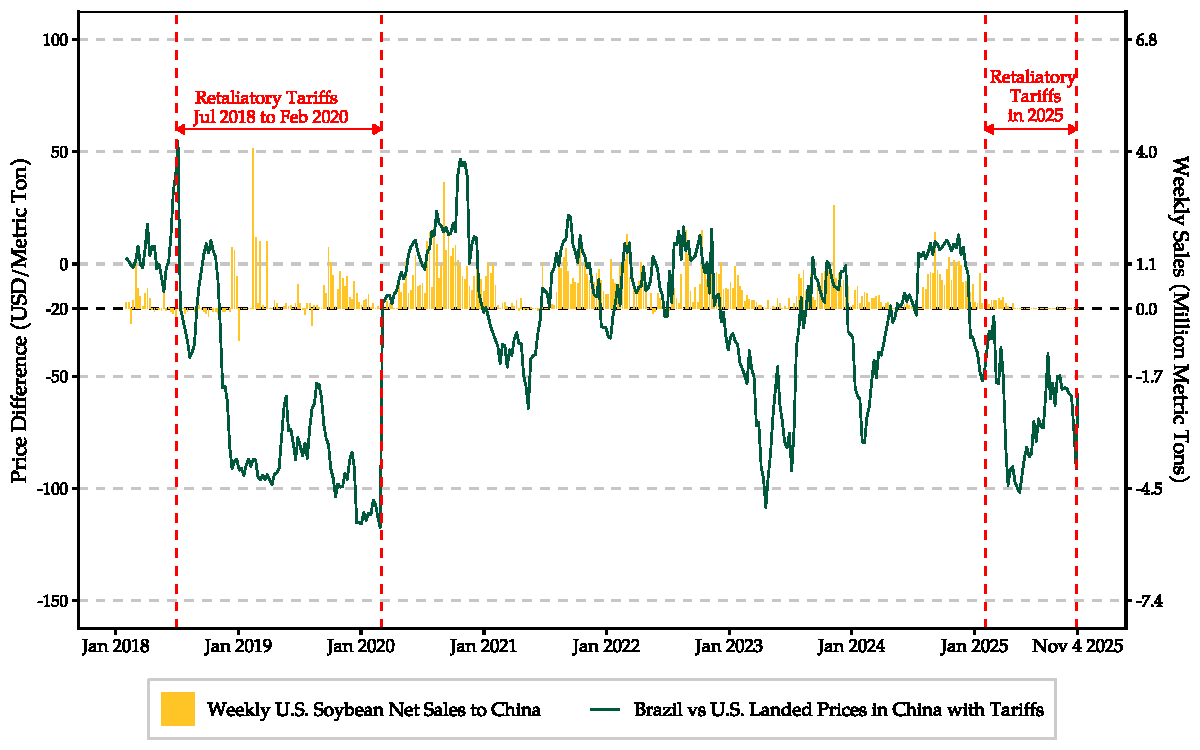
\includegraphics[width=0.95\linewidth]{visuals/figure2.pdf}
% --- notes/source, aligned to figure width ---
\vspace{3pt}
\begin{tablenotes}[flushleft]
\footnotesize
\setlength{\leftmargin}{0pt}      % remove item indentation
\setlength{\labelsep}{0pt}        % no gap before item text
\setlength{\itemsep}{4pt}         % vertical space between items
\setlength{\parsep}{0pt}          % no extra paragraph space
\setlength{\parindent}{0pt}       % no paragraph indent
\item \textit{Note:} Landed price in China includes shipping and insurance costs with tariffs (both MFN and retaliatory). The retaliatory tariff spike in April 2025 is not captured for presentation purposes.
\item \textit{Source:} DSU using data from Fastmarkets and USDA FAS Export Sales.
\end{tablenotes}

\end{threeparttable}
\end{figure}